% Modelo de Monografia (TCC) - UFAPE.
% No Overleaf/Prism, abra o main.tex e compile.
% Opções: arial (fonte Arial), notas (instruções do Word), frenteeverso (impressão dupla face).
\documentclass[monografia]{ufape}

% Dados
\autor{Nome do Aluno}
\titulo{Título da monografia}
\subtitulo{subtítulo}
\curso{xxxxxxxx}
\nomecurso{colocar o nome do curso} % opcional (se omitido, usa \curso)
\grau{Bacharelado ou Licenciatura}
\orientador{Prof. Dr. Xxxxxxxxxxxxxxxxx}
\cidade{Garanhuns}
\ano{2026}
% \dataaprovacao{15/12/2026} % padrão: ____/____/____
\logocurso{figuras/logo-curso.png} % troque pelo logo do curso ou apague a linha

% Banca (só nomes, sem assinaturas)
\membrobanca{Titulação. Nome Completo. (Orientador)}{Instituição a que pertence.}
\membrobanca{Titulação. Nome Completo do Membro da Banca.}{Instituição a que pertence.}
\membrobanca{Titulação. Nome Completo do Membro da Banca.}{Instituição a que pertence.}

% Parágrafo de exemplo do Word. Apague as chamadas e o comando ao escrever.
\newcommand{\textopadrao}{%
  A primeira linha de cada parágrafo terá recuo de 1,25~cm. Texto com fonte
  Times New Roman ou Arial, justificado, tamanho 12, espaçamento entre
  linhas de 1,5~cm (exceto para as citações diretas, no texto, com mais de
  três linhas, devem ser destacadas com recuo padronizado -- a ABNT NBR
  10520 recomenda que o recuo seja de 4~cm - em relação à margem esquerda,
  com letra menor que a utilizada no texto, em espaço simples e sem aspas.
  Para as citações diretas, no texto, com até três linhas, devem estar
  contidas entre aspas duplas), não colocar espaçamento entre parágrafos.\par}

\begin{document}

% Pré-textuais
\capa
\folhaderosto
\fichacatalografica

\begin{errata} % opcional: apague o ambiente se não houver errata
  \errataref{SOBRENOME, Prenome do Autor. \textbf{Título de obra}: subtítulo (se
    houver). Ano de depósito. Número de folhas. Monografia (Graduação). --
    Universidade Federal do Agreste de Pernambuco, Garanhuns, ano da defesa.}
  \tabelaerrata{16}{10}{auto-clavado}{autoclavado}
\end{errata}

\folhadeaprovacao

\begin{dedicatoria} % opcional
  Dedicatória é um elemento opcional. Deve ser inserida após a folha de
aprovação.

\end{dedicatoria}

\begin{agradecimentos} % opcional
  É um elemento \textbf{opcional}. Devem ser inseridos após a dedicatória. Esta folha é
conta, mas não se coloca a página. É nos agradecimentos que o autor retribui
às pessoas que contribuíram para a elaboração da monografia.

A primeira linha de cada parágrafo terá recuo de 1,25~cm. Texto com fonte
Times New Roman ou Arial, justificado, tamanho 12, espaçamento entre linhas
1,5~cm. Texto com fonte Times New Roman ou Arial, justificado, tamanho 12,
espaçamento entre linhas 1,5~cm.

A primeira linha de cada parágrafo terá recuo de 1,25~cm. Texto com fonte
Times New Roman ou Arial, justificado, tamanho 12, espaçamento entre linhas
1,5~cm. Texto com fonte Times New Roman ou Arial, justificado, tamanho 12,
espaçamento entre linhas 1,5~cm.

\end{agradecimentos}

\begin{epigrafe} % opcional
  A epígrafe é um elemento opcional. Esta folha é contada, mas não se coloca a
página. Não possui título e nem indicativo numérico. Elaborada conforme a ABNT
NBR 10520. Deve-se observar a quantidade de linhas que definirá o espaçamento
e a fonte. A epígrafe é uma citação direta de uma frase que pode ser ou não de
um autor conhecido e que diz respeito ao assunto abordado na monografia.
(Autor, ano, p. xx)

\end{epigrafe}

\begin{resumo}
  O resumo na língua vernácula é um elemento obrigatório e elaborado conforme a
ABNT NBR 6028. De acordo com a ABNT NBR 14724, todo o texto da monografia deve
ser digitado com espaçamento 1,5 entre linhas, \textbf{exceto} as citações de mais de
três linhas, notas de rodapé, referências, legendas das ilustrações e das
tabelas, natureza (tipo do trabalho, objetivo, nome da instituição a que é
submetido e área de concentração), que devem ser digitados ou datilografados
em espaço simples. As referências, ao final do trabalho, devem ser separadas
entre si por um espaço simples em branco. Texto com fonte Times New Roman ou
Arial, justificado, tamanho 12, espaçamento entre linhas 1,5~cm e conter de
150 a 500 palavras e sem citações. Texto com fonte Times New Roman ou Arial,
justificado, tamanho 12, espaçamento entre linhas 1,5~cm e conter de 150 a 500
palavras e sem citações. Texto com fonte Times New Roman ou Arial,
justificado, tamanho 12, espaçamento entre linhas 1,5~cm e conter de 150 a 500
palavras e sem citações. Texto com fonte Times New Roman ou Arial,
justificado, tamanho 12, espaçamento entre linhas 1,5~cm e conter de 150 a 500
palavras e sem citações. Texto com fonte Times New Roman ou Arial,
justificado, tamanho 12, espaçamento entre linhas 1,5~cm e conter de 150 a 500
palavras e sem citações.

\palavraschave{palavra; palavra; palavra.}

\nota{As palavras-chave devem ser grafadas com iniciais em letra minúscula, com
exceção dos substantivos próprios e nomes científicos, vir logo abaixo do
resumo, separadas por ponto e vírgula e finalizadas com ponto. No mínimo de 3
(três) e no máximo 5 (cinco) palavras-chave.}

\end{resumo}

\begin{abstract}
  O resumo em língua estrangeira é um elemento obrigatório e elaborado conforme
a ABNT NBR 6028. É a tradução do resumo na língua vernácula. De acordo com a
ABNT NBR 14724, todo o texto da monografia deve ser digitado com espaçamento
1,5 entre linhas, \textbf{exceto} as citações de mais de três linhas, notas de rodapé,
referências, legendas das ilustrações e das tabelas, natureza (tipo do
trabalho, objetivo, nome da instituição a que é submetido e área de
concentração), que devem ser digitados ou datilografados em espaço simples.
Texto com fonte Times New Roman ou Arial, justificado, tamanho 12, espaçamento
entre linhas 1,5~cm e conter de 150 a 500 palavras e sem citações. Texto com
fonte Times New Roman ou Arial, justificado, tamanho 12, espaçamento entre
linhas 1,5~cm e conter de 150 a 500 palavras e sem citações. Texto com fonte
Times New Roman ou Arial, justificado, tamanho 12, espaçamento entre linhas
1,5~cm e conter de 150 a 500 palavras e sem citações. Texto com fonte Times
New Roman ou Arial, justificado, tamanho 12, espaçamento entre linhas 1,5~cm e
conter de 150 a 500 palavras e sem citações. Texto com fonte Times New Roman
ou Arial, justificado, tamanho 12, espaçamento entre linhas 1,5~cm e conter de
150 a 500 palavras e sem citações.

\keywords{palavra; palavra; palavra.}

\nota{As palavras-chave devem ser grafadas com iniciais em letra minúscula, com
exceção dos substantivos próprios e nomes científicos, vir logo abaixo do
resumo, separadas por ponto e vírgula e finalizadas com ponto. No mínimo de 3
(três) e no máximo 5 (cinco) palavras-chave.}

\end{abstract}

\listadefiguras % opcional: apague se não houver figuras
\listadequadros % opcional: apague se não houver quadros
\listadetabelas % opcional: apague se não houver tabelas

\listadesiglas{% % opcional
  \item[ABNT] Associação Brasileira de Normas Técnicas
  \item[ONU] Organização das Nações Unidas
  \item[PNCRCL] Programa Nacional de Controle de Resíduos e Contaminantes em Leite
  \item[UFAPE] Universidade Federal do Agreste de Pernambuco
}

\listadesimbolos{% % opcional
  \item[\%] Percentual
  \item[\#] Hastag
  \item[@] Arroba
}

\sumario

% Textuais
\iniciotexto

\chapter{Introdução}
Nesta seção se aborda o tema do trabalho, a problemática da pesquisa, as
hipóteses, a justificativa, o objetivo geral e os específicos, a importância
da pesquisa para a comunidade científica e/ou sociedade, a metodologia de
pesquisa utilizada e uma rápida explanação do que trata cada seção da
monografia. A paginação da monografia inicia-se a partir desta página. A
introdução é uma seção primária.

Segue abaixo as normas da ABNT que são indispensáveis para a apresentação de
trabalhos científicos, de acordo com ABNT NBR 14724:

\begin{itemize}
  \item ABNT NBR 6023, Informação e documentação -- Referências -- Elaboração;
  \item ABNT NBR 6024, Informação e documentação -- Numeração progressiva das
        seções de um documento escrito -- Apresentação;
  \item ABNT NBR 6027, Informação e documentação -- Sumário -- Apresentação;
  \item ABNT NBR 6028, Informação e documentação -- Resumo -- Procedimento;
  \item ABNT NBR 6034, Informação e documentação -- Índice -- Apresentação;
  \item ABNT NBR 10520, Informação e documentação -- Citações em documentos --
        Apresentação;
  \item IBGE. Normas de apresentação tabular. 3. ed. Rio de Janeiro: IBGE, 1993.
        Disponível em:
        \url{https://biblioteca.ibge.gov.br/visualizacao/livros/liv23907.pdf}.
        Acesso em: 1 fev. 2022.
\end{itemize}

O texto escrito pelo autor ou as citações diretas até 3 linhas devem ser
digitado com espaçamento 1,5 entre as linhas, exceto se for citação direta com
mais de três linhas, notas de rodapé, referências, legendas das ilustrações e
das tabelas, natureza (tipo do trabalho, objetivo, nome da instituição a que é
submetido e área de concentração), que devem ser digitados em espaço simples.

\textopadrao


\chapter{Fundamentação teórica}
No desenvolvimento se detalha a pesquisa ou estudo realizado. É a parte mais
extensa da monografia. É no desenvolvimento que encontraremos a fundamentação
teórica, a metodologia, os resultados e a discussão.

Levando-se em consideração sobre estudos em acessibilidade em documentos
digitais, a escolha da fonte é uma decisão importante, pois é um elemento
imprescindível na monografia. Deve-se dar preferências as fontes sem serifa,
que são indicadas para leitura de documentos mais compreensível em word e PDF.

De acordo com Salton, Agnol e Turcatti (2017, p.~61),

\begin{citacaolonga}
É recomendada a utilização de fontes sem serifa (sans-serif), como Arial e
Verdana, uma vez que fontes serifadas podem dificultar a leitura de alguns
grupos de usuários, já que dão a impressão de estarem unidas devido aos
prolongamentos nos fins das hastes das letras. Da mesma forma, recomenda-se
evitar o uso de fontes muito elaboradas, decoradas e cursivas, que podem
confundir usuários com baixa visão e dificultar a leitura de pessoas com
dificuldades de aprendizagem.
\end{citacaolonga}

Segundo Brasil (2010, p.~17),

\begin{citacaolonga}
Fontes serifadas dão a impressão de estarem unidas, devido aos prolongamentos
no fim das hastes das letras, podendo confundir usuários com baixa visão. Além
disso, fontes muito ``enfeitadas'' dificultam a leitura de pessoas com
dificuldade de aprendizagem.
\end{citacaolonga}

As fontes sem serifa (\textit{Sans Serif}) são mais limpa como, por exemplo, a
fonte Arial. As fontes serifadas possuem um prolongamento no final das hastes
das letras que podem confundir os leitores de baixa visão, como por exemplo,
Times New Roman e Courier New.

O tipo de fonte para trabalhos acadêmicos não é especificada nas normas da
ABNT, mas as fontes indicadas e mais utilizadas são a Arial e a Times New
Roman, pois a diferença entre ambas é muito pouca.

\textopadrao

\textopadrao

\section{Seção Secundária}

A seção secundária é uma subdivisão do texto a partir de uma seção primária.
Para a elaboração das seções primárias, secundárias, terciárias, quaternárias
e quinárias, a autor deve seguir as orientações da ABNT NBR 6024 que trata
sobre a numeração progressiva. Esta norma destaca gradualmente os títulos das
seções e orienta na utilização dos recursos de negrito, itálico ou sublinhado
e outros. As seções que estão no sumário devem estar idênticas às seções que
estão no texto (ABNT, 2012).

As tabelas são formas não discursivas de apresentarem informações das quais o
dado numérico se destaca como informação central (tabela~\ref{tab:ibge}). A
formatação das tabelas segue as orientações do Instituto Brasileiro de
Geografia e Estatística (IBGE).

\vspace{15pt}
\begin{table}[H]
  \caption{Estudantes de curso superior de graduação, por tipo de curso superior de\\
    graduação que frequentavam, segundo as classes de rendimento mensal\\
    domiciliar e de rendimento mensal domiciliar per capita - Brasil -- 2014}
  \label{tab:ibge}
  \tabelaibge\raggedright
  \setlength{\tabcolsep}{0pt}\renewcommand{\arraystretch}{1}\setlength{\arrayrulewidth}{0.5pt}
  \noindent\hspace*{-0.7pt}\begin{tabular}{@{}p{139.8pt}*{6}{p{56.06pt}}@{}}
    \hline
    \multirow{4}{139.8pt}[-26pt]{\centering Classes de rendimento mensal domiciliar e de
      rendimento mensal domiciliar \textit{per capita}}
      & \multicolumn{6}{|c}{\rule[-6.2pt]{0pt}{15pt}Estudantes de curso superior de graduação} \\ \cline{2-7}
      & \multicolumn{3}{|c|}{\rule[-4.5pt]{0pt}{15pt}Valores absolutos (1\hspace{1.7pt}000 pessoas)}
      & \multicolumn{3}{c}{Valores relativos (\%)} \\ \cline{2-7}
      & \multicolumn{1}{|c|}{\multirow{2}{*}[-11pt]{\centering Total}}
      & \multicolumn{2}{c|}{\rule[-12pt]{0pt}{30pt}\begin{tabular}[c]{@{}c@{}}Tipo de curso superior de graduação\\ que frequentavam\end{tabular}}
      & \multicolumn{1}{c|}{\multirow{2}{*}[-11pt]{\centering Total}}
      & \multicolumn{2}{c}{\begin{tabular}[c]{@{}c@{}}Tipo de curso superior de graduação\\ que frequentavam\end{tabular}} \\ \cline{3-4}\cline{6-7}
      & \multicolumn{1}{|c|}{}
      & \multicolumn{1}{c|}{\rule[-12pt]{0pt}{30pt}\begin{tabular}[c]{@{}c@{}}Era superior de\\ tecnologia\end{tabular}}
      & \multicolumn{1}{c|}{\begin{tabular}[c]{@{}c@{}}Não era superior\\ de tecnologia\end{tabular}}
      & \multicolumn{1}{c|}{}
      & \multicolumn{1}{c|}{\begin{tabular}[c]{@{}c@{}}Era superior de\\ tecnologia\end{tabular}}
      & \multicolumn{1}{c}{\begin{tabular}[c]{@{}c@{}}Não era superior\\ de tecnologia\end{tabular}} \\ \hline
    \rule[-2.7pt]{0pt}{15pt}\hfill\textbf{Total}\hfill\null & \nc{7\hspace{1.7pt}242} & \nc{477} & \nc{6\hspace{1.7pt}765} & \nc{100,0} & \nc{100,0} & \nc{100,0} \\[9pt]
    \rule[-2.7pt]{0pt}{15pt}\hspace{3.7pt}\textbf{Classes de rendimento mensal domiciliar} & & & & & & \\
    \rule[-2.7pt]{0pt}{15pt}\hspace{10.7pt}Sem rendimento a 1 salário mínimo (1) & \nc{188} & \nc{11} & \nc{177} & \nc{2,6} & \nc{2,3} & \nc{2,6} \\
    \rule[-2.7pt]{0pt}{15pt}\hspace{10.7pt}Mais de 1 a 2 salários mínimos & \nc{612} & \nc{31} & \nc{581} & \nc{8,4} & \nc{6,5} & \nc{8,6} \\
    \rule[-2.7pt]{0pt}{15pt}\hspace{10.7pt}Mais de 2 a 3 salários mínimos & \nc{860} & \nc{51} & \nc{809} & \nc{11,9} & \nc{10,8} & \nc{12,0} \\
    \rule[-2.7pt]{0pt}{15pt}\hspace{10.7pt}Mais de 3 a 5 salários mínimos & \nc{1\hspace{1.7pt}664} & \nc{116} & \nc{1\hspace{1.7pt}547} & \nc{23,0} & \nc{24,4} & \nc{22,9} \\
    \rule[-2.7pt]{0pt}{15pt}\hspace{10.7pt}Mais de 5 a 10 salários mínimos & \nc{2\hspace{1.7pt}286} & \nc{166} & \nc{2\hspace{1.7pt}121} & \nc{31,6} & \nc{34,8} & \nc{31,3} \\
    \rule[-2.7pt]{0pt}{15pt}\hspace{10.7pt}Mais de 10 a 20 salários mínimos & \nc{914} & \nc{60} & \nc{854} & \nc{12,6} & \nc{12,6} & \nc{12,6} \\
    \rule[-2.7pt]{0pt}{15pt}\hspace{10.7pt}Mais de 20 salários mínimos & \nc{357} & \nc{15} & \nc{342} & \nc{4,9} & \nc{3,1} & \nc{5,1} \\
    \rule[-2.7pt]{0pt}{15pt}\hspace{10.7pt}Sem declaração & \nc{360} & \nc{26} & \nc{334} & \nc{5,0} & \nc{5,5} & \nc{4,9} \\
    \hline
  \end{tabular}\par
  \fonte[5.7pt]{IBGE (2014)}
\end{table}

\textopadrao

\textopadrao

\subsection{Seção Terciária}

A seção terciária é uma subdivisão do texto a partir de uma seção secundária.
Para a elaboração das seções primárias, secundárias, terciárias, quaternárias
e quinárias, a autor deve seguir as orientações da ABNT NBR 6024 que trata
sobre a numeração progressiva. Esta norma destaca gradualmente os títulos das
seções e orienta na utilização dos recursos de negrito, itálico ou sublinhado
e outros. As seções que estão no sumário devem estar idênticas às seções que
estão no texto (ABNT, 2012).

São consideradas ilustrações: os desenhos, esquema, fluxograma, fotografia,
gráfico, mapa, organograma, planta, quadro, retrato, figura, imagem, entre
outros. A identificação da ilustração é inserida na parte superior seguida de
seu número de ordem que se sucede dentro do texto, em algarismos arábicos,
travessão e do respectivo título. Na parte inferior da ilustração deve-se
colocar a fonte consultada. Caso necessite, após a fonte pode colocar legenda,
notas e outras informações. Deve-se citar no texto e inserir o mais próximo do
trecho a que se refere (ABNT, 2012).

Como exemplo, segue a figura~\ref{fig:1} abaixo.

\begin{figure}[H]
  \caption{Níveis do curso de Biblioteconomia na Biblioteca Nacional}
  \label{fig:1}
  \centering
  \begin{minipage}{225.6pt}
    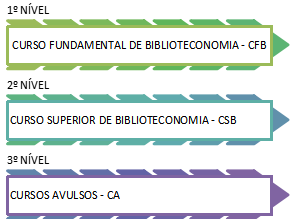
\includegraphics[width=225.6pt]{figuras/niveis-biblioteconomia.png}\par
    \fonte[4pt]{Elaborado pelos autores (2021).}
  \end{minipage}
\end{figure}

\textopadrao

\textopadrao

\subsubsection{Seção Quartenária}

A seção quaternária é uma subdivisão do texto a partir de uma seção terciária.
Para a elaboração das seções primárias, secundárias, terciárias, quaternárias
e quinárias, a autor deve seguir as orientações da ABNT NBR 6024 que trata
sobre a numeração progressiva. Esta norma destaca gradualmente os títulos das
seções e orienta na utilização dos recursos de negrito, itálico ou sublinhado
e outros. As seções que estão no sumário devem estar idênticas às seções que
estão no texto (ABNT, 2012).

\textopadrao

\textopadrao

\paragraph{Seção Quinária}

A seção quinária é uma subdivisão do texto a partir de uma seção quartenária.
Para a elaboração das seções primárias, secundárias, terciárias, quaternárias
e quinárias, a autor deve seguir as orientações da ABNT NBR 6024 que trata
sobre a numeração progressiva. Esta norma destaca gradualmente os títulos das
seções e orienta na utilização dos recursos de negrito, itálico ou sublinhado
e outros. As seções que estão no sumário devem estar idênticas às seções que
estão no texto (ABNT, 2012).

Os quadros possuem a mesma forma de apresentação das ilustrações. De forma
geral apresentam informações textuais, conforme o quadro~\ref{qua:normas}.

\vspace{3pt}
\begin{quadro}[H]
  \caption{Normas utilizadas na elaboração de um trabalho acadêmico}
  \label{qua:normas}
  \quadrotexto\raggedright
  \setlength{\tabcolsep}{5pt}\setlength{\arrayrulewidth}{0.5pt}
  \noindent\hspace*{20.9pt}\begin{tabular}{|>{\raggedright}p{39.6pt}|>{\raggedright}p{318.6pt}|>{\centering\arraybackslash}p{30.9pt}|}
    \hline
    \multicolumn{1}{|c|}{\textbf{Autor}} & \multicolumn{1}{c|}{\textbf{Título}} & \textbf{Ano} \\ \hline
    ABNT & NBR 6023, Informação e documentação -- Referências -- Elaboração. & 2018 \\ \hline
    ABNT & NBR 6024, Informação e documentação -- Numeração progressiva das seções de um documento escrito -- Apresentação. & 2012 \\ \hline
    ABNT & NBR 6027, Informação e documentação -- Sumário -- Apresentação. & 2012 \\ \hline
    ABNT & NBR 6028, Informação e documentação -- Resumo -- Procedimento. & 2021 \\ \hline
    ABNT & NBR 6034, Informação e documentação -- Índice -- Apresentação. & 2004 \\ \hline
    ABNT & NBR 10520, Informação e documentação -- Citações em documentos -- Apresentação. & 2023 \\ \hline
    IBGE & Normas de apresentação tabular & 1993 \\ \hline
  \end{tabular}\par
  \fonte[22.9pt]{Elaborado pelo autor (2021).}
\end{quadro}

\textopadrao

\textopadrao

\section{Seção Secundária}

A seção secundária é uma subdivisão do texto a partir de uma seção primária.
Para a elaboração das seções primárias, secundárias, terciárias, quaternárias
e quinárias, a autor deve seguir as orientações da ABNT NBR 6024 que trata
sobre a numeração progressiva. Esta norma destaca gradualmente os títulos das
seções e orienta na utilização dos recursos de negrito, itálico ou sublinhado
e outros. As seções que estão no sumário devem estar idênticas às seções que
estão no texto (ABNT, 2012).

\textopadrao

\textopadrao

\subsection{Seção Terciária}

A seção terciária é uma subdivisão do texto a partir de uma seção secundária.
Para a elaboração das seções primárias, secundárias, terciárias, quaternárias
e quinárias, a autor deve seguir as orientações da ABNT NBR 6024 que trata
sobre a numeração progressiva. Esta norma destaca gradualmente os títulos das
seções e orienta na utilização dos recursos de negrito, itálico ou sublinhado
e outros. As seções que estão no sumário devem estar idênticas às seções que
estão no texto (ABNT, 2012).

\textopadrao

\textopadrao

\subsubsection{Seção Quartenária}

A seção quaternária é uma subdivisão do texto a partir de uma seção terciária.
Para a elaboração das seções primárias, secundárias, terciárias, quaternárias
e quinárias, a autor deve seguir as orientações da ABNT NBR 6024 que trata
sobre a numeração progressiva. Esta norma destaca gradualmente os títulos das
seções e orienta na utilização dos recursos de negrito, itálico ou sublinhado
e outros. As seções que estão no sumário devem estar idênticas às seções que
estão no texto (ABNT, 2012).

\textopadrao

\textopadrao

\paragraph{Seção Quinária}

A seção quinária é uma subdivisão do texto a partir de uma seção quartenária.
Para a elaboração das seções primárias, secundárias, terciárias, quaternárias
e quinárias, a autor deve seguir as orientações da ABNT NBR 6024 que trata
sobre a numeração progressiva. Esta norma destaca gradualmente os títulos das
seções e orienta na utilização dos recursos de negrito, itálico ou sublinhado
e outros. As seções que estão no sumário devem estar idênticas às seções que
estão no texto (ABNT, 2012).

\textopadrao

\textopadrao


\chapter{Metodologia}
Nesta seção o autor vai descrever os métodos e materiais que foram utilizados
para a elaboração do trabalho. É na metodologia que o autor encontrará
respostas para as questões como? com quê? onde? quanto?.

Na metodologia o autor descreve o método de abordagem, os materiais utilizados
e as técnicas para a coleta dos dados.

\textopadrao

\textopadrao


\chapter{Resultados e análise dos dados}
Nesta seção o autor apresenta e discuti os principais resultados.

\textopadrao

\textopadrao


\chapter{Considerações finais}
Esta seção é a parte final da monografia onde o autor discorre sobre suas
conclusões referentes ao tema estudado. Trata-se da síntese da exposição dos
dados e dos exemplos tratados nas seções anteriores.

É na conclusão que o autor vai informar se os objetivos foram alcançados, se
foi esclarecido o problema de pesquisa, se as hipóteses foram confirmadas ou
negadas, descrever as dificuldades encontradas na pesquisa, informar à
contribuição que o trabalho trouxe para a sociedade ou comunidade científica
e, se houver, recomendações e/ou sugestões para futuros trabalhos referentes
ao tema abordado.

\textopadrao

\textopadrao


% Pós-textuais
\begin{referencias}
  \refitem{ASSOCIAÇÃO BRASILEIRA DE NORMAS TÉCNICAS. \textbf{NBR 6024}: informação
e documentação: numeração progressiva das seções de um documento: apresentação.
Rio de Janeiro: ABNT, 2012.}

\refitem{ASSOCIAÇÃO BRASILEIRA DE NORMAS TÉCNICAS. \textbf{NBR 14724}:
informação e documentação: trabalhos acadêmicos: apresentação. Rio de Janeiro:
ABNT, 2011.}

\refitem{BRASIL. Tribunal de Contas da União. \textbf{Criando documentos digitais
acessíveis}. Brasília: TCU, 2010. Disponível em:
\url{https://www.tjdft.jus.br/acessibilidade/publicacoes/producao_de_conteudo_com_acessibilidade_vf3.pdf}.
Acesso em: 14 dez. 2021.}

\refitem{NASCIMENTO, Maria Vanessa do.; MARTINS, Graci Kelly. A trajetória das
escolas de biblioteconomia no Brasil. \textbf{REBECIN}: Revista Brasileira de
Educação em Ciência da Informação, São Paulo, v.4, n. esp., p. 37-54, 2. sem.,
2017. Disponível em: \url{https://portal.abecin.org.br/rebecin/article/view/90}.
Acesso em: 14 dez. 2021.}

\refitem{SALTON, Bruna Poletto; AGNOL, Anderson Dall; TUCARTTI, Alissa.
\textbf{Manual de acessibilidade em documentos digitais}. Bento Gonçalves:
Instituto Federal de Educação, Ciência e Tecnologia do Rio Grande do Sul, 2017.}

\refnota{O autor deve descrever todas as referências que foram citadas dentro da monografia.
As referências devem ser alinhadas à esquerda e com espaçamento simples. São
organizadas em ordem alfabética por sobrenome dos autores. Entre cada
referência, deve ter uma linha em branco com espaço simples, de acordo com a
NBR 6023/2018.}

\end{referencias}

\apendice{A}{Título} % opcional
Esta seção trata sobre apêndice que é um texto ou documento elaborado pelo
autor da monografia para completar o trabalho.

Se o documento tiver alguma assinatura, essas devem ser ocultadas. Tanto nesta
parte, como em qualquer outra do trabalho.


\apendice{B}{Título} % opcional
Esta seção trata sobre apêndice que é um texto ou documento elaborado pelo
autor da monografia para completar o trabalho.

Se o documento tiver alguma assinatura, essas devem ser ocultadas. Tanto nesta
parte, como em qualquer outra do trabalho.


\anexo{A}{Título} % opcional
Esta seção trata do anexo que é um texto ou documento que não foi produzido
pelo autor da monografia. O texto ou documento que está anexado ao trabalho
deve servir de fundamentação, comprovação e ilustração, como por exemplo:
mapas, leis, estatutos, etc.

Se o documento tiver alguma assinatura, essas devem ser ocultadas. Tanto nesta
parte, como em qualquer outra do trabalho.


\anexo{B}{Título} % opcional
Esta seção trata do anexo que é um texto ou documento que não foi produzido
pelo autor da monografia. O texto ou documento que está anexado ao trabalho
deve servir de fundamentação, comprovação e ilustração, como por exemplo:
mapas, leis, estatutos, etc.

Se o documento tiver alguma assinatura, essas devem ser ocultadas. Tanto nesta
parte, como em qualquer outra do trabalho.


\end{document}
